\documentclass{sbc2023}%

\usepackage{graphicx}
\usepackage{listings}
%\usepackage[utf8]{inputenc}
\usepackage[misc,geometry]{ifsym} 
\usepackage{fontspec}
\usepackage{fontawesome}
\usepackage{academicons}
\usepackage{color}
\usepackage{hyperref} 
\usepackage{aas_macros}
\usepackage[bottom]{footmisc}
\usepackage{supertabular}
\usepackage{afterpage}
\usepackage{url}
\usepackage{pifont}
\usepackage{multicol}
\usepackage{multirow}
\usepackage[brazil]{babel}
\lstset{
    basicstyle=\ttfamily\small,  
    commentstyle=\color{codegreen},
    keywordstyle=\color{blue},
    numberstyle=\tiny\color{codegray},
    stringstyle=\color{codepurple},
    breaklines=true,
    keepspaces=true,                 
    numbers=left,
    frame=single,
    xleftmargin=0pt,
    xrightmargin=0pt,
    aboveskip=1em,
    belowskip=1em,
    captionpos=b
}

\setcitestyle{square}

\definecolor{orcidlogo}{rgb}{0.37,0.48,0.13}
\definecolor{unilogo}{rgb}{0.16, 0.26, 0.58}
\definecolor{maillogo}{rgb}{0.58, 0.16, 0.26}
\definecolor{darkblue}{rgb}{0.0,0.0,0.0}
\hypersetup{colorlinks,breaklinks,
            linkcolor=darkblue,urlcolor=darkblue,
            anchorcolor=darkblue,citecolor=darkblue}
%\hypersetup{colorlinks,citecolor=blue,linkcolor=blue,urlcolor=blue}

%%%%%%% IMPORTANT: We disable hyperlinks by default with this line, to avoid the error "\pdfendlink ended up in different nesting level" while writing.
%\hypersetup{draft}

\jid{JBCS}
\jtitle{Journal of the Brazilian Computer Society, 2025}
\copyrightstatement{This work is licensed under a Creative Commons Attribution 4.0 International License}
\jyear{2025}

\title[Análise de Custo Computacional da Busca de Imagens Coloridas]{Análise de Custo Computacional da Busca de Imagens Coloridas em Diferentes Estruturas de Dados}

%THE ORCID IS MANDATORY FOR EACH AUTHOR IN JBCS
\author[Viterbo et al. 2025]{
\affil{\textbf{André Mendes Rodrigues}~[\textbf{Pontíficia Universidade Católica de Minas Gerais}]~[\textbf{1405342@sga.pucminas.br}]}

\affil{\textbf{Arthur Martinho M. Oliveira}~[\textbf{Pontíficia Universidade Católica de Minas Gerais}]~[\textbf{1109821@sga.pucminas.br}]}

\affil{\textbf{Caio Gomes A. Glória}~[\textbf{Pontíficia Universidade Católica de Minas Gerais}]~[\textbf{1379601@sga.pucminas.br}]}

\affil{\textbf{Daniel Salgado Magalhães}~[\textbf{Pontíficia Universidade Católica de Minas Gerais}]~[\textbf{1470797@sga.pucminas.br}]}

\affil{\textbf{Nilson Deon C. Filho}~[\textbf{Pontíficia Universidade Católica de Minas Gerais}]~[\textbf{1369636@sga.pucminas.br}]}
}

\begin{document}

\begin{frontmatter}
\maketitle

\begin{mail}
Instituto de Ciências Exatas e Informática, R. Dom José Gaspar, 500 - Coração Eucarístico, Belo Horizonte - MG, 30535-901 
\end{mail}

\begin{abstract}
\textit{~Este trabalho aborda o problema de busca de documentos semelhantes representados como imagens. Cada imagem é modelada como um vetor de características com base em suas principais cores. Três estruturas de dados diferentes foram implementadas para suportar a busca por similaridade: lista sequencial, quadtree e tabela hash. O objetivo é analisar e comparar os custos computacionais dessas abordagens. Os resultados demostraram as relações precisão/eficiência de cada estrutura, destacando as limitações da busca sequencial em comparação à quadtree e hash.}
\noindent 
\end{abstract}

\begin{keywords}
Custo Computacional, Estruturas de Dados, Lista, Hash, Quadtree, Análise de Algoritmos
\end{keywords}

%\begin{license}
%Published under the Creative Commons Attribution 4.0 International Public License (CC BY 4.0)
%\end{license}

\end{frontmatter}

\section{Introdução}
\label{sec:intro}
O trabalho consiste na análise de custo computacional em operações de busca de imagens coloridas em estruturas de dados diferentes. As imagens foram mapeadas como documentos representados como um vetor de características, e a busca realizada retorna documentos que sejam semelhantes ao documento escolhido para consulta.

Neste trabalho foram abordadas e analisadas três diferentes tipos de estruturas de dados, sendo elas, a Lista, a Hash, e a Quadtree. O objetivo do trabalho com estas estruturas é analisar, de forma prática e teórica, quais são as diferenças entre cada uma delas em relação à forma de execução e custo de tempo.

A execução de cada uma das estrutura de dados foi chamada na \textit{main}, assim como a função para carregar a imagem escolhida para consulta. A lista e a hash realizaram a análise de vetores a partir da ferramenta Qui-Quadrado ($x^2$), que determina se existe uma associação significativa entre variáveis, neste caso, entre histogramas. A quadtree usa uma simplificação dos dados da imagem (a matiz média e a saturação média) como coordenadas para organizar o espaço.

\section{Lista}
A lista é, na teoria e na prática, a mais simples de ser implementada, e a menos eficiente em termos de resultados. A lista de forma básica realiza uma busca de forma linear entre elementos, percorrendo cada um dos elementos para comparar o vetor da posição ao vetor de consulta.

A complexidade de tempo desta busca linear é O(n), já que ela verifica todos os elementos presentes na estrutura de dados para realizar todas as comparações. Porém, no código a lista foi ordenada para que os elementos estivessem em posição sequencial ordenada, de forma que uma busca binária fosse possível, transformando a complexidade de busca em O(log(n)). Como cada vetor de características é multidemensional, devido à conversão das imagens para um vetor através do processo do descritor, estes vetores foram lidos como histogramas, para uso da ferramenta Qui-Quadrado.

A função que calcula a distância entre os histogramas é iniciada com uma variável de distância total com valor zero. Em seguida, um laço \textit{for} percorre cada posição, denominada de \textit{bin}, dos histogramas simultaneamente. A cada iteração, primeiro é calculada a diferença entre os valores dos dois histogramas naquele \textit{bin} específico, e o resultado é elevado ao quadrado. Isso garante que o valor seja sempre positivo e penaliza diferenças grandes de forma mais precisa que as pequenas.

Depois, para normalizar essa diferença, o valor ao quadrado é dividido pela soma dos valores dos dois histogramas naquele mesmo \textit{bin}. Isso dá um peso maior para as diferenças que ocorrem em \textit{bins} com valores menores. O resultado dessa divisão é então somado à variável de distância total. Após o término do laço \textit{for}, o valor acumulado na distância total é multiplicado por 0.5 para obter o resultado final, conforme a fórmula padrão da distância Qui-quadrado.

\begin{center}
\begin{lstlisting}[language=c++ ,caption = Cálculo entre histogramas na Lista]
inline float chi2_distance(const std::vector<float>& h1, const std::vector<float>& h2) {
    float dist = 0.0f;
    for (size_t i = 0; i < h1.size(); i++) {
        float num = (h1[i] - h2[i]) * (h1[i] - h2[i]);
        float den = h1[i] + h2[i] + 1e-8;
        dist += num / den;}
    return 0.5f * dist;}
\end{lstlisting}
\end{center}

\section{Quadtree}
A Quadtree é uma estrutura de dados utilizada principalmente para particionar o espaço bidimensional em regiões menores. Seu funcionamento tem como base a divisão recursiva de uma área em quatro quadrantes, de modo que cada nó da árvore possui até quatro filhos. No contexto do trabalho, a Quadtree foi utilizada para indexar imagens a partir das características extraídas de seus descritores. Cada imagem é representada como um ponto no espaço bidimensional. Assim, imagens com características cromáticas parecidas tendem a ocupar regiões próximas na árvore.

A implementação da classe Quadtree segue um modelo de divisão espacial. Cada nó é associado a uma região retangular (\textit{Rect}), definida dentro de cada um, e os descritores são armazenados até que a capacidade máxima seja atingida. Quando isso ocorre, o nó é subdividido em quatro quadrantes menores, criados por meio de ponteiros, e os pontos subsequentes passam a ser distribuídos entre esses nós filhos.

O processo de inserção é realizado pela função \textit{insert}, que verifica inicialmente se o ponto pertence à região delimitada pelo nó. Para a consulta, o método \textit{queryRange} percorre a árvore recursivamente, mas apenas nas regiões que interceptam o retângulo de busca especificado. Essa estratégia permite restringir a busca a uma fração do espaço, evitando varreduras completas como na lista sequencial.

Em termos de complexidade, a Quadtree apresenta um custo de O(n*log n), embora no pior caso tenha complexidade de O(n) quando os pontos ficam concentrados em poucas regiões. Ainda assim, a estrutura mostra-se bem eficiente, principalmente quando os descritores de imagens são projetados em um espaço bidimensional.

\begin{center}
\begin{lstlisting}[language=c++ ,caption = Estrutura de ponto para análise na Quadtree]
struct Point {
    float x, y; // muH, muS
    Record record;
};

struct Rect {
    float x, y;     // centro
    float halfW, halfH; // metade da largura e altura
    bool contains(const Point& p) const {
        return (p.x >= x - halfW && p.x <= x + halfW &&
                p.y >= y - halfH && p.y <= y + halfH);
    }
    bool intersects(const Rect& range) const {
        return !(range.x - range.halfW > x + halfW ||
                 range.x + range.halfW < x - halfW ||
                 range.y - range.halfH > y + halfH ||
                 range.y + range.halfH < y - halfH);
    }
};
\end{lstlisting}
\end{center}

\section{Hash}
A ideia central da Tabela Hash implementada é associar cada imagem a uma chave hash derivada de suas características de cor extraídas. O objetivo é que imagens com descritores visualmente semelhantes sejam mapeadas para o mesmo \textit{bucket} na tabela, mesmo que seus histogramas completos não sejam idênticos. A principal vantagem da Tabela Hash é sua capacidade de realizar buscas em tempo médio constante, ou seja, com complexidade de tempo de O(1).

Isso é possível através de uma função de hash que mapeia o vetor de características a uma posição específica (um \textit{bucket}) na tabela. Ao buscar por uma imagem, a mesma função de hash é aplicada ao vetor de consulta, e o sistema verifica apenas os vetores armazenados no \textit{bucket} correspondente.

No processo de inserção, cada imagem é carregada e seu descritor de características, contendo um histograma de cores HSV, é extraído. Este descritor é então processado pela função \textit{makeHashKey}, que cria uma “assinatura de cor” simplificada ao identificar a matiz (\textit{Hue}) dominante, o nível médio de saturação (\textit{Saturation}) e de brilho (\textit{Value}). Essa assinatura, uma \textit{string} como “7-1-2”, serve como a chave da tabela. O registro da imagem é inserido na tabela hash, e colisões, vistas como múltiplas imagens com a mesma assinatura, são tratadas naturalmente, agrupando todos os registros correspondentes em um mesmo bucket, que é uma lista.

Na etapa de consulta, a imagem de entrada passa pelo mesmo processo: seu descritor é gerado e a função \textit{makeHashKey} produz a chave do \textit{bucket} alvo. A busca é então otimizada, restringindo-se inicialmente apenas aos registros desse \textit{bucket}. Caso o número de candidatos seja insuficiente, a implementação adota uma estratégia de \textit{fallback}, coletando registros de outros \textit{buckets} para garantir um conjunto robusto para a comparação. Os registros candidatos são então avaliados de forma precisa através da distância Qui-quadrado ($x^2$) entre seus histogramas completos e o da consulta. Por fim, os resultados são ordenados pelo grau de similaridade (menor distância) e os K melhores são retornados.

No pior caso, onde todas as chaves geram o mesmo valor de hash, a complexidade é O(n), onde “n” é o número de itens na tabela, sendo o pior dos casos. Porém, de maneira geral, a busca em uma tabela hash é realizada em tempo O(1), o que representa uma vantagem significativa em relação à busca sequencial em uma lista.

\begin{center}
\begin{lstlisting}[language=c++ ,caption = Cálculo entre histogramas na Hash]
inline std::string makeHashKey(const Descriptor& d) {
    // Hue dominante (0..7)
    int hBin = 0;
    float maxVal = -1.0f;
    for (int i = 0; i < 8; i++) { // primeiros 8 bins correspondem ao Hue
        float val = 0.0f;
        for (int s = 0; s < 3; s++) {
            for (int v = 0; v < 3; v++) {
                int idx = i * (3 * 3) + s * 3 + v;
                val += d.hist[idx];
            }
        }
        if (val > maxVal) {
            maxVal = val;
            hBin = i;
        }
    }

    // Saturação média → 0=baixa,1=média,2=alta
    int sBin = (d.muS < 0.33) ? 0 : (d.muS < 0.66 ? 1 : 2);

    // Value médio aproximado: vamos pegar bins de V somando ao longo do histograma
    float meanV = 0.0f;
    float total = 0.0f;
    for (int h = 0; h < 8; h++) {
        for (int s = 0; s < 3; s++) {
            for (int v = 0; v < 3; v++) {
                int idx = h * 9 + s * 3 + v;
                meanV += v * d.hist[idx];
                total += d.hist[idx];
            }
        }
    }
    meanV /= (total + 1e-8);
    int vBin = (meanV < 1.0) ? 0 : (meanV < 2.0 ? 1 : 2);

    return std::to_string(hBin) + "-" + std::to_string(sBin) + "-" + std::to_string(vBin);
}
\end{lstlisting}
\end{center}

\section{Resultados}
Os testes finais foram realizados com aproximadamente 4000 imagens a fim de comparar o desempenho, e os resultados mostraram diferenças no tempo total de execução entre as três estruturas. A base de dados possui imagens coloridas de diferentes cores, testando poucas imagens com focos em paisagens de certas cores e depois, com uma variedade maior de cores, verificando as diferenças de resultados presentes. 

De forma geral, foi possível perceber que como a comparação da imagem é feita por cálculo do histograma, imagens que poderiam ser parecidas em questão de conteúdo, não seriam necessariamente as imagens escolhidas. Porém, na questão das cores em si, os resultados foram positivos e as cores parecidas com as da imagem escolhida.

A lista apresentou o pior desempenho, com 21.350 segundos. 


\begin{figure}[h]
    \centering
    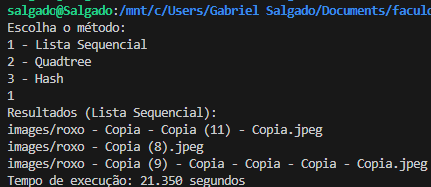
\includegraphics[width=0.45\textwidth]{lista2.png}
    \caption{Lista sequencial}
    \label{fig:exemplo}
\end{figure}

A Quadtree obteve um tempo total de 18.765 segundos, representando uma redução considerável em relação à lista.


\begin{figure}[ht]
    \centering
    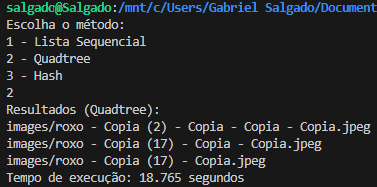
\includegraphics[width=0.45\textwidth]{quadtree2.png}
    \caption{Quadtree}
    \label{fig:exemplo}
\end{figure}

Já a estrutura Hash apresentou o melhor desempenho entre as três, com 18.276 segundos, beneficiando-se do acesso esperado em tempo constante aos buckets. 


\begin{figure}[ht]
    \centering
    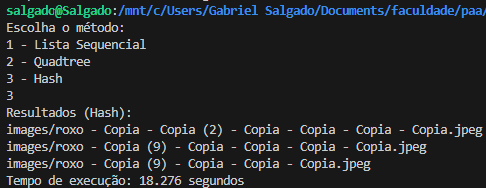
\includegraphics[width=0.45\textwidth]{hash2.png}
    \caption{Tabela Hash}
    \label{fig:exemplo}
\end{figure}

Esses resultados confirmam a análise de que estruturas de indexação espacial são mais adequadas do que a abordagem sequencial para problemas de recuperação de imagens em bases de grande volume.

\begin{figure}[ht]
    \centering
    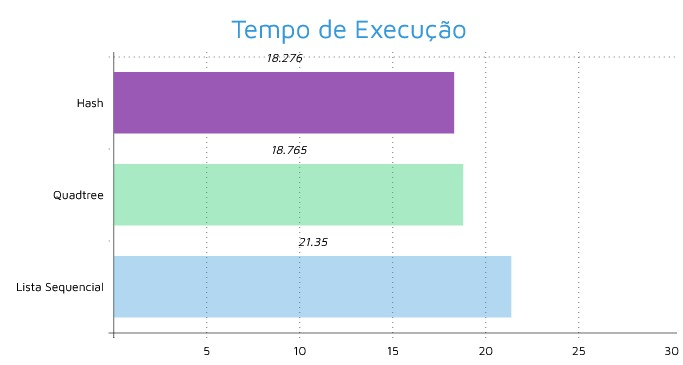
\includegraphics[width=0.5\textwidth]{grafico.jpeg}
    \caption{Tempos de Execução}
    \label{fig:exemplo}
\end{figure}

\section{Conclusão}
A partir das análises realizadas nesse trabalho, é possível concluir que as diferentes implementações de estruturas de dados impactam diretamente na velocidade e custo computacional referentes ao retorno da busca. A lista, apesar de ser a mais fácil de implementar, é a primeira a decair em questão de perfomance e tempo a medida que a base de dados vai aumentando. Em testes menores, ela conseguiu equivaler ao tempo das outras estruturas, porém com o aumento da base de dados, a diferença entre elas foi ficando maior, mesmo que um método de ordenação para pesquisa binária tivesse sido implementado. A quadtree implementada possui os resultados médios entre as 3 estruturas, ficando no meio entre o mais eficiente (Hash) e menos eficiente (Lista). A divisão por quadrantes facilitou bastante a busca, devido as partições realizadas, entretanto, a busca entre essa partições foi demonstrada como mais custosa que a busca do algoritmo mais eficiente. Por fim, a Hash possui os melhores resultados, sendo a mais eficiente para os resultados e custo computacional, entre as 3 estruturas analisadas. O aumento da base de dados pode ser gerenciado com a implementação de técnicas como o Hashing Sensível à Localidade (LSH), conseguindo manejar a alta dimensionalidade com métodos de busca de vizinhos.

Dessa forma, é possível notar que a quantidade da base de dados influencia significativamente no retorno das estruturas de dados. Entretanto, acima disso, a forma como cada estrutura realiza a busca tem uma influência maior. É possível que no futuro, outras estruturas de dados sejam implementadas para verificar tempos e custos mais eficientes que o da Hash com técnica de LSH.

\bibliographystyle{apalike-sol}

\begin{thebibliography}{99}
\bibitem{sciencedirect_computational_analysis}
ScienceDirect,  
\textit{Computational Analysis},  
Artigo online, disponível em: \url{https://www.sciencedirect.com/topics/engineering/computational-analysis}.

\bibitem{clubedogis_quadtree}
Clube do GIS,  
\textit{O que é Quadtree em GIS -- Estruturas de Dados},  
disponível em: \url{https://clubedogis.com.br/glossario/o-que-e-quadtree-em-gis-estruturas-de-dados/}.

\bibitem{croco_quadtree}
Adriano Croco,  
\textit{Analisando algoritmos: QuadTree},  
Medium (artigo online), publicado em 15 fev. 2024, disponível em: \url{https://42bits.medium.com/analisando-algoritmos-quadtree-2fe86394f624/}.

\bibitem{harley_quadtree}
Aldo von Wangenheim e Harley Wagner,  
\textit{QuadTree},  
UFSC (artigo online), publicado em 1998, disponível em: \url{https://www.inf.ufsc.br/~aldo.vw/visao/1998/harley/quadtree.htm}.

\bibitem{video_hash_estruturaDados}
Canal: Paulo Paraluppi,  
\textit{Tabelas Hash - Estrutura de Dados - Unicamp},  
Vídeo no YouTube, publicado em 22 abril. 2011, disponível em: \url{https://www.youtube.com/watch?v=Non0I_OSt9o&t=2s}.

\bibitem{youtube_hash_funcao_introducao}
Canal: Professor Douglas Maioli,  
\textit{Aula 08 Estrutura de Dados - Tabela Hash - Introdução},  
Vídeo no YouTube, publicado em 16 mar. 2021, disponível em: \url{https://www.youtube.com/watch?v=5pYYy3Z0m9I}.

\end{thebibliography}

\end{document}
